\documentclass{article}%
\usepackage[T1]{fontenc}%
\usepackage[utf8]{inputenc}%
\usepackage{lmodern}%
\usepackage{textcomp}%
\usepackage{lastpage}%
\usepackage[head=40pt,margin=0.5in,bottom=0.6in]{geometry}%
\usepackage{graphicx}%
%
\title{\textbf{¿Maduro censura el mensaje del papa Francisco?}}%
\author{EL NACIONAL WEB}%
\date{16/09/2018}%
%
\begin{document}%
\normalsize%
\maketitle%
\textbf{URL: }%
http://www.el{-}nacional.com/noticias/iglesia/maduro{-}censura{-}mensaje{-}del{-}papa{-}francisco\_251957\newline%
%
\textbf{Periodico: }%
EN, %
ID: %
251957, %
Seccion: %
Iglesia\newline%
%
\textbf{Palabras Claves: }%
Política\newline%
%
\textbf{Derecho: }%
CONTEXTO, %
Otros Derechos: %
, %
Sub Derechos: %
\newline%
%
\textbf{EP: }%
NO\newline%
\newline%
%
\textbf{\textit{Los obispos de Venezuela denunciaron en el Vaticano que el gobierno venezolano quiere desarrollar una política anti eclesiástica en los medios de comunicación}}%
\newline%
\newline%
%
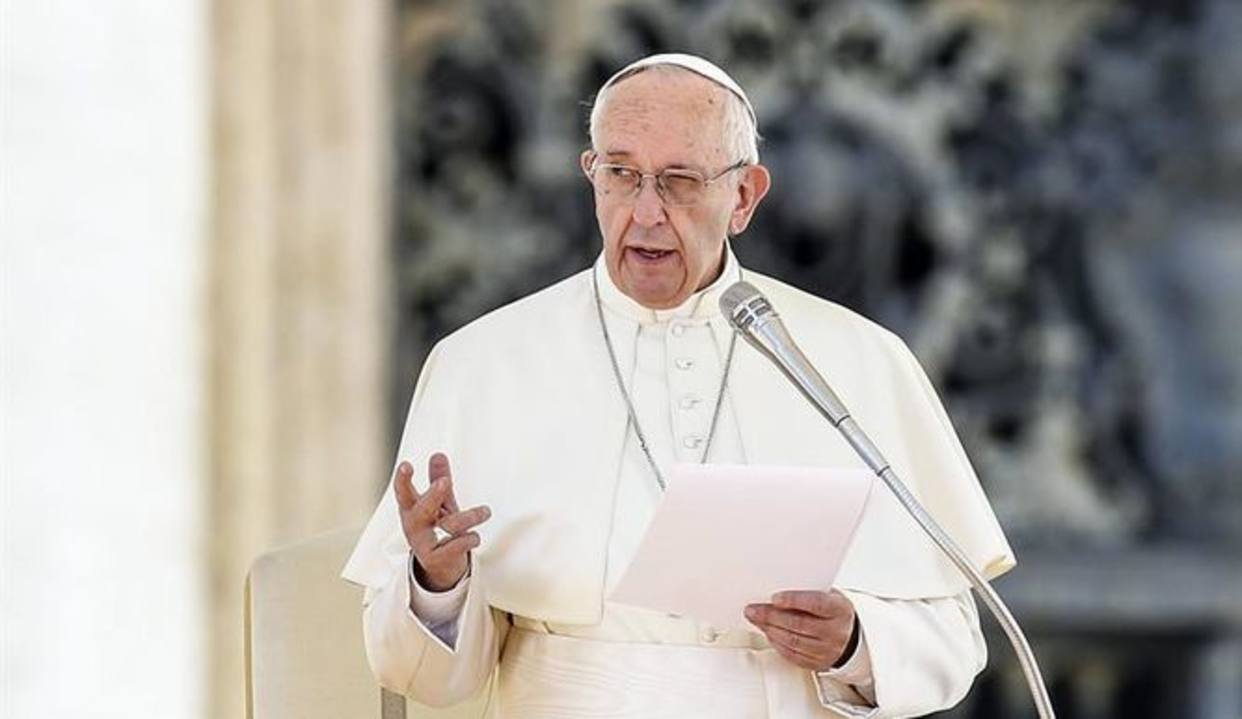
\includegraphics[width=300px]{179.jpg}%
\newline%
%
El papa Francisco agradeció este martes a los obispos venezolanos por su resistencia durante~una reunión en el Vaticano. Sin embargo, los mensajes que envió el pontífice~a la población venezolana no han tenido mayor resonancia, más allá de los círculos allegados a la iglesia, reseñó~Aleteia.%
\newline%
%
El periodista Ramón Antonio Pérez explicó que, a su juicio, esto se debe a que el presidente Nicolás Maduro tiene control absoluto en los medios de comunicación, los cuales están obligados a cumplir con las reglas impuestas por el gobierno.%
\newline%
%
Pérez expresó que los religiosos venezolanos~denunciaron en el Vaticano que el gobierno de~Maduro quiere desarrollar una política anti eclesiástica en los medios de comunicación.%
\newline%
%
“Se está viviendo un fuerte proceso de recentralización del poder político y mediático del Estado y una marcada tendencia a la ideologización y a la intolerancia, por parte del gobierno nacional, en todos los ámbitos de la sociedad, particularmente en el de los medios de comunicación social”, indicó el informe que fue enviado a Francisco antes de la visita de los representantes venezolanos.%
\newline%
%
El informe señaló que la Comisión Nacional de Telecomunicaciones (Conatel) se encarga de confiscar equipos periodísticos cuando consideran que no cumplen con los lineamientos ideológicos del gobierno de Maduro.%
\newline%
%
Respecto a la relación del pontífice con los representantes de la iglesia en Venezuela, el monseñor Mario Moronta indicó que: “¡El papa Francisco no es comunista!~Algunos están deseando que el papa diga que nosotros~(los obispos venezolanos) estamos en contra de él”.%
\newline%
%
Lea más en~Aleteia.%
\newline%
%
\end{document}